\section{Evaluation}\label{sec:evaluation}

We evaluate the six properties of Section~\ref{sec:claims} against ca2a 0.3.1, then the current
release (commit \texttt{7d90823}, September 26, 2026); 0.4.0 followed on October 1, 2026
(Section~\ref{sec:after}). Every experiment in this section was rerun
on September 27, 2026. The original July 2026 results came from an earlier, unpinned checkout;
where numbers changed, both are reported.

\subsection{Environment and reproducibility}

The experiments ran under CPython 3.12.10 (an x86-64 build running under emulation on a Windows
11 laptop with an ARM64 Snapdragon X1E80100 processor), with dependencies from the project's
runtime lock at that commit: \texttt{cryptography} 50.0.1, \texttt{cedarpy} 4.8.7,
\texttt{agent-manifest} 0.12.0, \texttt{agentrust-trace} 0.10.0, and \texttt{rfc8785} 0.1.4. The
one deviation from the lock is \texttt{cbor2} 5.9.0 in place of 6.1.4, because the host's
application-control policy blocks the 6.x native extension. Timings are single runs under
emulation and vary from run to run; they show how cost scales, not what a server would measure.
No hardware TEE is needed. The rerun record, with every command's output, is committed with the
paper as \texttt{experiments/results/rerun-2026-09-27.txt}.

Two sets of experiments are used. The repository's own per-claim experiments live under
\texttt{experiments/} in ca2a~\citep{ca2arepo2026}; the three scale and cost experiments below
ship with this report and import the runtime from a ca2a checkout named by \texttt{CA2A\_ROOT}:

\begin{lstlisting}[language=bash,caption={Rerunning the experiments}]
# in a ca2a checkout at tag v0.3.1
pip install -e ".[dev]"
python experiments/claim1-attenuation-soundness/run.py   # C1 .. claim6 likewise
# in this report's directory
CA2A_ROOT=/path/to/ca2a python experiments/c1_attenuation_scale.py
CA2A_ROOT=/path/to/ca2a python experiments/verify_latency_vs_depth.py
CA2A_ROOT=/path/to/ca2a python experiments/sealed_channel_throughput.py
\end{lstlisting}

At 0.3.1, \texttt{verify\_chain} refuses a chain whose root issuer the caller has not named as
trusted (ca2a commit \texttt{23c980a}), so the three report scripts now pass each chain's root as
the trusted set; no other logic changed. The project's test suite at the same commit produced 779
passes and 11 skips: nine skips need a git checkout rather than the source archive used here, and
two need hardware captures. Setting \texttt{CA2A\_TDX\_QUOTE} to a genuine GCP Intel TDX quote
published in the agent-manifest repository ran one of those two: the TDX verifier appraised it to
the pinned Intel SGX Root CA, and all 17 TDX tests passed. That is offline appraisal of one
captured quote, not a live attested call. Table~\ref{tab:ca2a-results} summarizes the outcomes.

\begin{table}[h]
\centering
\caption{Outcomes at ca2a 0.3.1, rerun September 27, 2026. The Status column names the layer at
which each property was checked.}
\label{tab:ca2a-results}
\small
\begin{tabular}{>{\raggedright\arraybackslash}p{3.3cm}>{\raggedright\arraybackslash}p{2.6cm}>{\raggedright\arraybackslash}p{8.2cm}}
\toprule
Property & Status & Result \\
\midrule
C1 Attenuation soundness & Validated (software) & 200/200 narrowing chains accepted and 200/200 escalations rejected with \texttt{ScopeEscalation}; across depths 2 to 8, 2500/2500 accepted and 2500/2500 rejected \\
C2 In-chain replay and splice & Validated (software) & Duplicate \texttt{credential\_id} raises \texttt{CredentialReplay}; cross-chain splice raises \texttt{BrokenDelegationLink}; 2/2 controls valid \\
C3 Scope-policy intersection & Validated (software) & Effective scope is delegated $\cap$ local policy; 1/1 allowed, 3/3 denied; the inbound transport tests exercise the same decision \\
C4 Sealed-payload confidentiality & Cryptographic layer & 4/4: only the peer's key opens the payload; the path sees ciphertext; wrong key and tamper fail closed. Key confinement to attested code not shown \\
C5 Provenance integrity & Structural (experiment) & Tampering one record changed 119 and 138 of 256 hash bits in two runs and raised \texttt{ProvenanceLinkBroken}; reparenting detected; record $i$ bound to credential $i$ \\
C6 Cross-operator attestation & Synthetic evidence & 4/4 with synthetic SEV-SNP vectors: independent keys, mutual appraisal, sealed delegation, binary swap rejected. No hardware run across independent operators \\
\bottomrule
\end{tabular}
\end{table}

\subsection{C1: Attenuation Soundness}
\label{sec:eval-c1}

\textbf{Setup.} Property~\ref{prop:c1} states that a child grant can never exceed its parent.
The repository experiment generates 200 independent four-hop delegation chains. In the narrowing
case, each hop drops exactly one capability from a six-capability root, so every hop is a strict
subset of the one above it. In the escalating case, the third hop adds a fresh capability that no
ancestor held. Each chain is signed hop by hop, so issuer continuity, depth, and
\texttt{parent\_id} linkage hold; only the scope relationship differs.

\textbf{Results.} All 200 narrowing chains are accepted, and all 200 escalating chains are
rejected with \texttt{ScopeEscalation}; none is rejected by an unrelated error. A correctly
signed credential that widens its scope is still rejected, so attenuation is enforced
independently of signature validity.

\textbf{Across chain depth.} For each depth in $\{2,3,4,6,8\}$ we generated 500 narrowing chains
and 500 escalation chains (each escalation injects a never-held capability at an interior hop)
over a 16-capability root universe, 2500 of each in total. Every narrowing chain was accepted and
every escalation was rejected with \texttt{ScopeEscalation}, with zero rejections by an unrelated
error, matching the July result. The per-depth counts are in
\texttt{experiments/results/c1\_attenuation\_scale.json}.

\subsection{Verification Latency vs Chain Depth}
\label{sec:eval-latency}

\textbf{Setup.} Chain verification is the per-call cost a callee pays before it acts: trusted
root, signature, validity, continuity, attenuation, and in-chain replay over every hop. We built
one correctly signed chain at each depth in $\{1,2,4,8,16,32,64\}$, ran 200 warm-up iterations,
then timed \texttt{verify\_chain} over 2000 iterations per depth, reporting mean, p50, and p99.
Chains are signed once up front, so the measurement excludes key generation.

\textbf{Results.} Cost grows linearly with depth, at about 216 microseconds per hop between depth
1 and depth 64 (July: about 195). A single hop verifies in 0.25\,ms mean; a 64-hop chain verifies
in 13.87\,ms mean with p99 26.08\,ms (July: 0.14\,ms, 12.45\,ms, and 22.15\,ms).
Table~\ref{tab:rerun-compare} lists both runs, and Figure~\ref{fig:latency-depth} plots the rerun.
The two runs differ in code version (the verifier gained trusted-root and validity-window checks
after July) and in environment, so the difference is not attributed to either alone. At realistic depths of a few
hops the cost stays near a millisecond or below. Raw values are in
\texttt{experiments/results/verify\_latency\_vs\_depth.json}.

\begin{table}[h]
\centering
\caption{Original (July 1, 2026, unpinned checkout) and rerun (September 27, 2026, ca2a 0.3.1)
timings. Both are single runs on developer hardware.}
\label{tab:rerun-compare}
\small
\begin{tabular}{lrr}
\toprule
Measurement & July 2026 & Rerun \\
\midrule
\texttt{verify\_chain}, depth 1, mean (ms) & 0.14 & 0.25 \\
\texttt{verify\_chain}, depth 8, mean (ms) & 1.73 & 2.07 \\
\texttt{verify\_chain}, depth 64, mean / p99 (ms) & 12.45 / 22.15 & 13.87 / 26.08 \\
Slope, depth 1 to 64 ($\mu$s per hop) & 195 & 216 \\
Seal and open, 64 bytes, round trip (ms) & 0.21 & 0.17 \\
Seal and open, 256\,KiB, throughput (MiB/s) & 266 & 212 \\
\bottomrule
\end{tabular}
\end{table}

\begin{figure}[h]
\centering
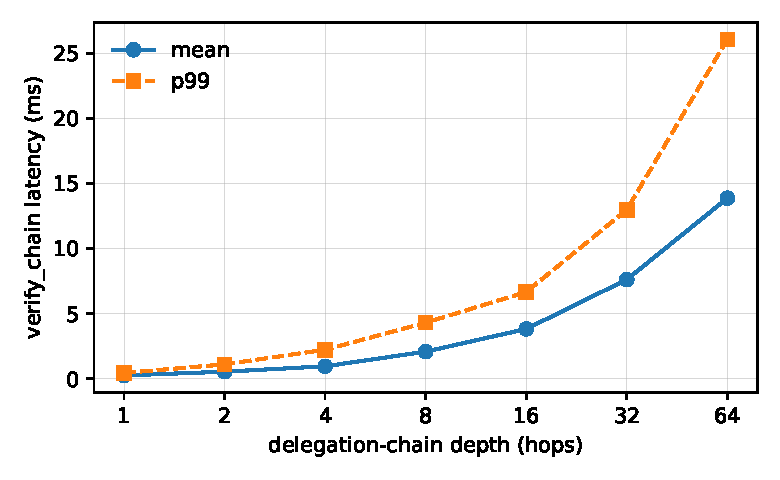
\includegraphics[width=0.62\linewidth]{figures/verify_latency_vs_depth.pdf}
\caption{Chain-verification latency (mean and p99) versus delegation-chain depth, log-scale
x-axis, 2000 timed iterations per depth, ca2a 0.3.1. Cost is linear in depth at about 216
microseconds per hop; a 64-hop chain verifies in 13.87\,ms mean.}
\label{fig:latency-depth}
\end{figure}

\subsection{C2: In-Chain Replay and Splice Rejection}
\label{sec:eval-c2}

\textbf{Setup.} Property~\ref{prop:c2} states that a credential replayed within a chain or
spliced from another chain is rejected. We build two independent, well-formed chains, A and B,
each with its own key material and credential-id namespace. Three cases are checked: (1) a
control in which both chains verify unmodified; (2) an intra-chain replay in which one hop's
\texttt{credential\_id} is duplicated inside the chain; and (3) a cross-chain splice in which a
validly signed credential minted for chain A is inserted into chain B.

\textbf{Results.} Both control chains verify (2/2). The duplicated \texttt{credential\_id} raises
\texttt{CredentialReplay}. The spliced credential is rejected with \texttt{BrokenDelegationLink}
because its \texttt{parent\_id} does not match chain B's preceding credential. A valid signature is
therefore necessary but not sufficient; continuity is enforced over the chain, not per
credential. Replay of a whole valid chain by a different party is outside this experiment; the
project covers it with holder-proof tests.

\subsection{C3: Scope-Policy Intersection}
\label{sec:eval-c3}

\textbf{Setup.} Property~\ref{prop:c3} states that the capability a caller may exercise against a
peer is the intersection of its verified delegated scope with the callee's local policy. We build
a two-hop chain delegating a leaf scope of \{\texttt{read}, \texttt{write}\} (the root also held
\texttt{admin}) and set the callee's local policy to allow \{\texttt{read}, \texttt{audit}\}. We
then request four capabilities through \texttt{effective\_scope} and \texttt{enforce\_peer\_call}:
\texttt{read} (delegated and allowed), \texttt{write} (delegated but not locally allowed),
\texttt{audit} (locally allowed but never delegated), and \texttt{admin} (neither).

\textbf{Results.} The effective scope is exactly \{\texttt{read}\}. Only \texttt{read} is allowed
(1/1); \texttt{write}, \texttt{audit}, and \texttt{admin} are each denied with
\texttt{ScopeNotPermitted} (3/3). A capability is exercised only when the chain granted it
\emph{and} the local policy permits it. The experiment uses the set-based \texttt{LocalPolicy};
the project's unit tests exercise the Cedar engine, and its live-call and \texttt{a2a-sdk}
loopback tests, which passed in the rerun, drive the same decision through an inbound HTTP and
JSON-RPC request on the local host, including a denial for an out-of-scope capability. None of
these is a deployment across a real network boundary.

\subsection{C4: Sealed-Payload Confidentiality}
\label{sec:eval-c4}

\textbf{Setup.} Property~\ref{prop:c4} states that a sealed task payload decrypts only with the
private key matching the peer's appraised channel key. The peer generates a channel keypair; we
seal a secret payload to its public key with \texttt{ca2a\_runtime.channel} and check four
sub-properties: (1) the sealed blob does not contain the plaintext; (2) the peer's private key
recovers it; (3) an unrelated key cannot open it; and (4) a tampered ciphertext fails closed
under AEAD authentication.

\textbf{Results.} All four checks pass (4/4). A different key and a flipped byte both raise
\texttt{SealedChannelError} rather than returning corrupted plaintext. This validates payload
confidentiality at the cryptographic layer. It says nothing about whether the peer's host can read
the private key; that is the hardware dependency Property~\ref{prop:c4} names, and
Section~\ref{sec:after} reports platform state that bears on it.

\textbf{Throughput and latency.} We measured the sealed channel across payload sizes from a
64-byte task envelope to a 256\,KiB document, timing \texttt{seal} (ephemeral key generation,
ECDH, HKDF, AEAD encryption) and \texttt{open} (ECDH, HKDF, AEAD decryption) over 2000 iterations
each after warm-up, with a round-trip check confirming every opened payload equalled the
original. A 64-byte envelope seals and opens in 0.17\,ms round trip, a cost dominated by the fixed
X25519 and HKDF setup. As payloads grow the setup amortizes and the AEAD dominates: end-to-end
throughput rises from 0.37\,MiB/s at 64 bytes to 212\,MiB/s at 256\,KiB (July: 0.21\,ms and
266\,MiB/s). Figure~\ref{fig:sealed-throughput} plots the rerun. Raw measurements are in
\texttt{experiments/results/sealed\_channel\_throughput.json}.

\begin{figure}[h]
\centering
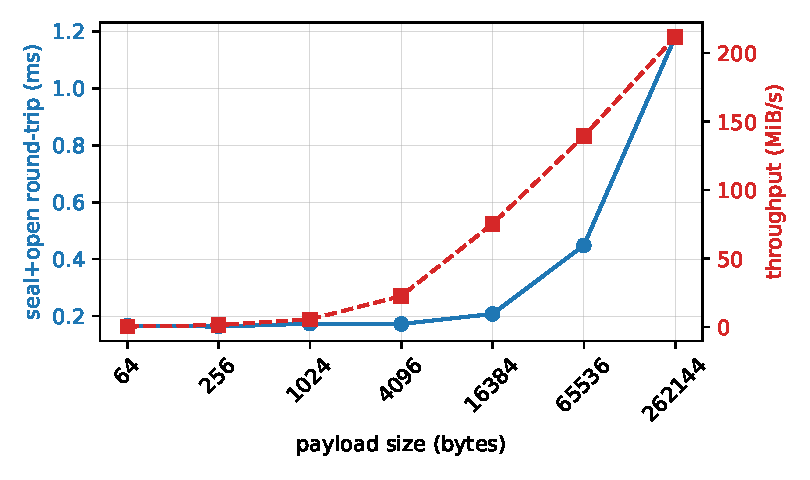
\includegraphics[width=0.64\linewidth]{figures/sealed_channel_throughput.pdf}
\caption{Sealed-channel round-trip latency (left axis) and end-to-end throughput (right axis)
versus payload size, log-scale x-axis, 2000 timed \texttt{seal} and \texttt{open} iterations per
size, ca2a 0.3.1. Small payloads are setup-dominated (0.17\,ms round trip at 64 bytes); large
payloads are AEAD-dominated, reaching 212\,MiB/s at 256\,KiB.}
\label{fig:sealed-throughput}
\end{figure}

\subsection{C5: Provenance Integrity}
\label{sec:eval-c5}

\textbf{Setup.} From a signed three-hop chain the repository experiment emits one unsigned
\texttt{DelegationRecord} per hop, each carrying the SHA-256 \texttt{record\_hash} of its parent.
It checks four sub-properties: (1) a valid record set verifies with \texttt{verify\_dag}; (2)
changing a record's scope changes its \texttt{record\_hash} and breaks its child's parent link;
(3) pointing a record at the wrong ancestor is detected; and (4) \texttt{cross\_check\_chain}
binds record $i$ to credential $i$.

\textbf{Results.} The valid record set verifies. Injecting one capability into a record's scope
changed 119 and 138 of the 256 bits of its \texttt{record\_hash} in two runs, as expected of
SHA-256~\citep{avalanche1985}, and \texttt{verify\_dag} raised \texttt{ProvenanceLinkBroken}
because the child's stored parent hash no longer matched. Reparenting the leaf record was likewise
detected, and \texttt{cross\_check\_chain} raised \texttt{ProvenanceLinkBroken} when a record's
\texttt{credential\_id} was forged.

\textbf{What this shows.} These records are unsigned, so the experiment shows structural
consistency against a single edit, not authenticity: a writer who rewrites every record can
recompute every link and pass all four checks, and an edit to the leaf has no child link to
break. Authenticity comes from the signed TRACE path (\texttt{verify\_trace\_dag} and
\texttt{cross\_check\_trace\_dag}), whose unit tests, including those binding each record's
signing key to the chain's delegate, passed in the rerun. That path is not measured by a separate
experiment in this report.

\subsection{C6: Cross-Operator Attestation}
\label{sec:eval-c6}

\textbf{Setup.} The repository experiment builds two operators, each with its own channel keypair
and its own synthetic VCEK key, and binds each channel key into a synthetic SEV-SNP report. Both
synthetic VCEK certificates chain to one synthetic root standing in for the AMD ARK. Each side
verifies the other's report chain and signature with the shipped verifier, checks the
measurement against an expected value, seals a delegated task to the key the report binds, and
finally presents a validly signed report with a different measurement.

\textbf{Results.} All four checks pass (4/4): the keys are independent, each report's channel key
is recovered after verification, the sealed task opens only with the peer's key, and the report
with the swapped measurement is rejected with \texttt{AttestationFailed}. This exercises the
protocol logic and the verifier code. It does not show that genuine hardware produces such
reports for this protocol between independent operators. The recorded hardware runs
(Section~\ref{subsec:attestation}) were one-directional across two clouds or mutual within one
operator, their raw evidence is not published, and they were not repeated for this edition. C6
therefore remains unvalidated on hardware.
